\noindent For the remainder of the paper, we present a detailed investigation 
into the performance implications of the locality-exploiting optimizations on a 
number of representative unstructured-mesh applications. The applications are 
all well established in literature and are representative of several domains 
that make use of unstructured mesh codes. Our aim is to present the performance 
of the state-of-the-art on GPUs with these applications and then contrast the 
performance gained with our contributions. 

\subsection{Experimental setup}\label{experimental-setup}

\noindent The GPU systems used in performance analysis is detailed in 
Table~\ref{tab:GPU_datasheet}. These consist of two of NVIDIAs latest 
high-performance computing Tesla GPUs, namely the P100 and V100. The GPUs are 
hosted in a server with an Intel Xeon CPU E5-1660 (3.20GHz base frequency, 1 
socket with 8 cores) running Ubuntu 16.04. The nvcc compiler with CUDA version 
9.0 (V9.0.176) is used. 
\begin{table}
\centering
\begin{tabular}{lcc}
\hline
  & P100 (GP100) & V100 (GV100)\\ \hline\hline
  Streaming Multiprocessors (SM) 		& 56	& 80\\ \hline
  Max Thread Block Size				& 1024	& 1024 \\ \hline
  Max Warps / Multiprocessor 			& 64 & 64	\\ \hline
  Max Threads / Multiprocessor		& 2048 & 2048	\\ \hline
  Max Thread Blocks / Multiprocessor 	& 32 & 32	\\ \hline
  Max Registers / Thread& 255 & 255	\\ \hline
  Shared Memory Size / SM	& 64 KB & 96 KB	\\ \hline
  Max 32 - bit Registers / SM			& 65536 & 65536\\ \hline
  Memory Size							& 16 GB	& 16 
GB\\ \hline
  L2 Cache Size						& 4096 KB & 6144 KB\\ 
\hline
  Peak Stream Bandwidth					& 495 GB/s & 742 GB/s\\ 
\hline
\end{tabular}
  \caption{Important informations about the NVIDIA Tesla P100 and V100 GPUs
  \cite{Pascal_whitepaper, Volta_whitepaper}}
\label{tab:GPU_datasheet}
\end{table}

Both runtime performance as well as low-level metrics on the GPUs such as 
achieved bandwidth and occupancy is utilized to understand the bottlenecks 
affecting performance. There are three key factors of interest: (1) 
the coloring approach (global or hierarchical) giving the best performance, 
(2) method of data reordering (no-reordering, GPS-based, or graph 
partitioning-based) and (3) data layout (AoS or SoA). All combinations of these 
are evaluated and compared to each other and a state-of-the-art reference 
implementation.

When comparing performance of different versions, we use the achieved bandwidth
as the key performance metric. Emphasis on bandwidth is justified given that 
all of the test applications, as we demonstrate, are memory-bound. Achieved 
bandwidth is calculated by the formula: $$\frac{\sum_{d} w_dS_d}{T} \cdot I,$$ 
where $d$ iterates over the datasets, $w_d$ is $2$ if the data is read and 
written, $1$ otherwise, $S_d$ is the size of the dataset (in bytes), $T$ is the 
overall runtime of the kernel and $I$ is the number of iterations. A number 
of additional metrics were also collected, these include:
\begin{itemize}
\item data reuse factor (the average number of times an indirectly accessed
data point is accessed),
\item the number of read/write transactions from/to global memory, which is
closely related to the data reuse factor but is affected by memory access
patterns, and therefore cache line utilization,
\item the occupancy reflecting the number of threads resident on the SM versus
the maximum - the higher this is, the better chance of hiding the latency of
compute/memory operations and synchronization
\item the percentage of stalls occurring because of data requests, execution
dependencies, or synchronization,
\item the number of block colors; the higher it is, the less work in a
single kernel launch, which tends to lead to lower utilization of the GPU,
\item the number of thread colors; the higher this is the more
synchronizations are required to apply the increments in shared memory ---
but also strongly correlates with data reuse,
\item warp execution efficiency (ratio of the average active threads per warp
to the maximum number of threads per warp).
\end{itemize}
Studying runtime performance and the above metrics enables us to understand 
and explain why certain variants are better than others.


\subsubsection{Airfoil}

\noindent Airfoil, implemented using the OP2 DSL~\cite{op2} is the smallest, 
best understood and most thoroughly studied among the applications we explored. 
It is representative of large industrial Finite Volume CFD applications and 
implements a non-linear 2D inviscid airfoil code using an unstructured grid. A 
finite-volume discretization is used to solve the 2D Euler equations with a 
scalar numerical dissipation. The algorithm iterates towards the steady state 
solution, in each iteration using a control volume approach, meaning the change 
in the mass of a cell is equal to the net flux along the four edges of the cell, 
which requires indirect connections between cells and edges. Two versions of the 
code exists, one implemented with OP2's C/C++ API and the other using OP2's 
Fortran API~\cite{giles2012op2,op2-repo}.

The application consists of five parallel loops in total: \texttt{save\_soln}, 
\texttt{adt\_calc}, \texttt{res\_calc}, \texttt{bres\_calc} and \texttt{update}.
Here we focus on \texttt{res\_calc}, as it has indirect increments and about 
70\% of the total runtime of the application is spent in this parallel loop on 
GPUs when using a global coloring. The loop contains both indirect reads and 
writes. It iterates through edges (i.e. the from-set), and computes the flux 
through edges using data accessed indirectly on the two cells adjacent to each 
edge. The \texttt{res\_calc} loop is called 2000 times during the  
execution of the application and performs about 100 floating-point operations 
per mesh edge. In each iteration, it reads 5 and increments 4 double values from 
each of the 2 indirectly accessed cells, and reads 2 double values from each of 
the 2 indirectly accessed nodes. 

Table \ref{tab:airfoil_counters_glob} show the effect of various optimizations 
on the Airfoil application's \texttt{res\_calc} kernel, during the execution on 
a mesh with 2.8 million cells.


\begin{table}[Htbp]
\centering
\resizebox{\columnwidth}{!}{
\begin{tabular}{|R{3cm}|cc|c|c||cc|c|c||c|}\hline
Coloring  & \multicolumn{4}{c||}{Global} & \multicolumn{4}{c||}{Hierarchical} & 
\begin{tabular}{@{}c@{}}Original \\ Hierarchical\end{tabular}\\\hline
Reordering & \multicolumn{2}{c|}{none} & GPS & partition & 
\multicolumn{2}{c|}{none} & \multicolumn{2}{c||}{partition} & none\\\hline
Data layout &    AOS      &   SOA     &     SOA      &    SOA & AOS      &   SOA 
    &     AOS      &    SOA & SOA\\\hline
Bandwidth (GB/s)&  $72$ & $94$ &  $106$&  $66$&    $ 211$ &   $ 215$ &
$ 228$ &   $ 239$ & $ 233$\\\hline
Runtime (ms) & $6.12$ & $4.65$ & $4.15$ & $6.64$ & $2.07$ & $2.03$ & $1.92$ & 
$1.83$ & $1.91$\\\hline
Achieved Occupancy&  $0.63$ &  $0.45$ &      $0.45$&            $0.45$&    
$0.44$ &   $0.52$ &      $0.59$ &   $0.42$ & $0.42$\\\hline
Global Memory Read Transactions&  \num{52424}k & \num{45781}k & \num{41246}k& 
\num{66775}k& \num{21142}k & \num{21192}k & \num{13964}k & \num{14406}k& 
\num{21866}k\\\hline
Global Memory Write Transactions& \num{14007}k & \num{14737}k & \num{13773}k& 
\num{20733}k& \num{5807}k  & \num{57883}k & \num{3397}k  & \num{3669}k & 
\num{6384}k\\\hline
Number of (Block) Colours&  $5$&  $5$ &      $5$ &            $7$&    $       4$ 
&   $       4$ &      $       8$ &   $       8$ &   $       5$\\\hline
Number of Thread Colours&-&-&-&-&    $       3$ &   $       3$ &      $       4$ 
&   $       4$ &   $       3$\\\hline
Reuse Factor&-&-&-&-&    $       2$ &   $       2$ &      $     3.6$ &   $     
3.6$ &   $       2$\\\hline
Issue Stall Reasons (Synchronization)&-&-&-&-&    $  11\%$ &   $   9\%$ &      $ 
 14\%$ &   $  14\%$ &   $  14\%$\\\hline
Issue Stall Reasons (Data Request)&-&-&-&-&    $  69\%$ &   $  68\%$ &      $  
61\%$ &   $  63\%$ &   $  55\%$\\\hline
Block Size &\multicolumn{8}{c||}{$480$} &   $128$\\\hline
\end{tabular}
}
\caption{Low-level performance metrics of Airfoil's \texttt{res\_calc} kernel - 
global coloring vs hierarchical coloring (2.8 million mesh cells). The last 
column details the measured performance of the original code.}
\label{tab:airfoil_counters_glob}
\end{table}


\emph{Global coloring}: We see that using the SoA layout improves performance. 
As discussed in Section~\ref{aos-to-soa}, with SoA threads in a warp access data 
addresses that are near each other. The improvement can also be seen in 
the number of global memory read transactions as it is roughly $87\%$ of that 
with AoS layout. Adding the GPS renumbering improves performance 
further by placing data points that are accessed in consecutive threads close 
to each other. Now there is a $19\%$ reduction in global read transactions 
compared to the baseline AoS. Given that the partition based reordering is 
primarily intended for the hierarchical coloring, it does not improve on the 
Global coloring. The reason being that partitioning groups threads 
that access the same data together, while the global coloring puts them into 
different kernel launches, eliminating any chance for spatial reuse.

\emph{Hierarchical coloring:}  The key goal of this strategy is to better 
exploit data reuse by using the GPU shared memory. The effectiveness of the 
approach show immediately due to the significant reduction in the number of 
global transactions in Table~\ref{tab:airfoil_counters_glob}. At block size 
$480$, there is roughly a $60\%$ decrease in global read and write 
transactions, leading to three times the performance. Throughput for different 
block sizes is shown in Figure~\ref{fig:airfoil_bw-vs-bs_hier_large}.

We also see that reordering using partitioning is indeed more effective. With
a block size of 448, data reuse increases from $2$ on the reference version,
to $3.6$, leading to the $19\%$ performance gain over the version without
reordering (AoS layout). This is also consistent with the number of global
transactions: there is a $35\%$ decrease in the number of reads and $41\%$
decrease in the number of writes, and a decrease in the percentage of stalls
occurring because of data requests: $61\%$ with partitioning, $68\%$ without.

With the increased reuse, the number of thread colors is also larger ($4$
versus $2.2$) and this leads to more synchronization. With reordering, $14\%$
of the stalls were caused by synchronization, up from $9\%$. This is further 
illustrated by Figure \ref{fig:airfoil_speedup_large} that shows the relative 
speedup compared to the original OP2 version (its low-level metrics are detailed 
in the final column of Table~\ref{tab:airfoil_counters_glob}). In this case, the 
original version also used the shared memory approach, so the performance gains 
are caused by the reordering. In the original version (hierarchical coloring, SOA
layout) $56\%$ of the total time is spent in \texttt{res\_calc}. The best original
version used the SOA data layout, with reordering we achieved $19\%$ speedup on
\texttt{res\_calc} with AOS layout.
However with AOS layout we lose performance in direct kernels, therefore regarding
the whole application one can reach better performance with the SOA layout.
The best performing setting of airfoil reached about $3.3\%$ speedup on the whole 
application. The useful bandwidth of the best performing version of 
\texttt{res\_calc} (our implementation) reached $55\%$ of the peak stream bandwidth
of the P100 GPU. 
%Although the number of block colors increased with reordering, we believe that this is due to the 
% problem size, where there are too few blocks of the of the same color to 
% saturate the GPU. 


\begin{figure}[Htbp]
\centering
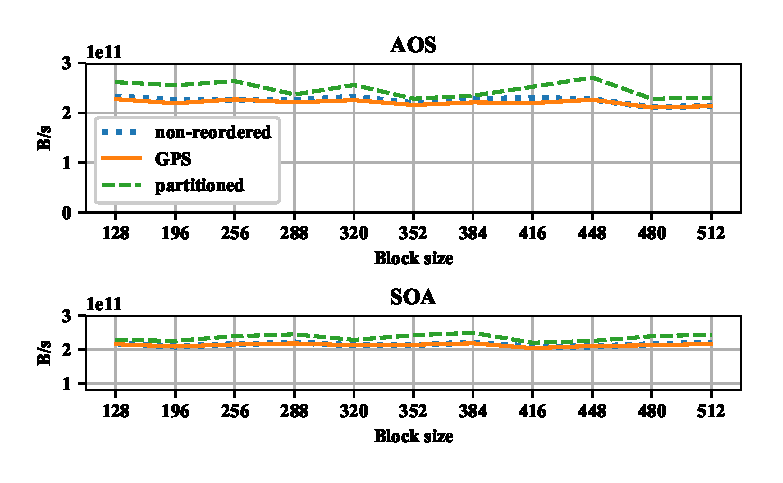
\includegraphics[width=10cm]{fig/airfoil_bw-vs-bs_hier_large.eps}
\caption{Airfoil's \texttt{res\_calc} bandwidth on a dataset with $2880000$ 
cells with hierarchical coloring.}
\label{fig:airfoil_bw-vs-bs_hier_large}
\end{figure}

\begin{figure}[Htbp]
\centering
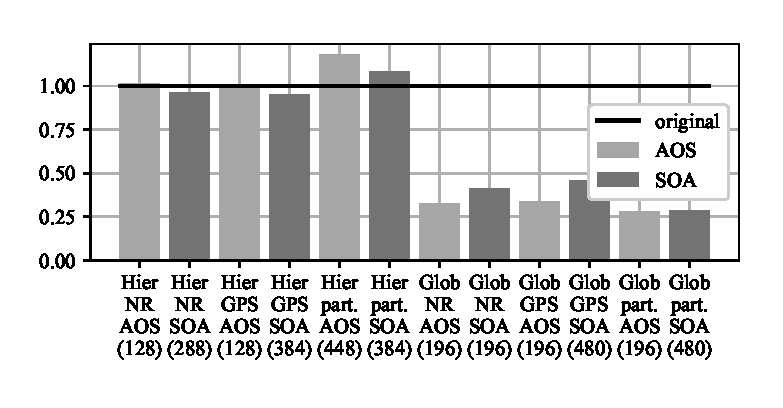
\includegraphics[width=10cm]{fig/airfoil_speedup_large.eps}
\caption{Airfoil's \texttt{res\_calc} kernel speedup compared to the original 
code (on a mesh with $2800000$ cells. The block sizes are shown in parentheses, 
the reordering algorithms are: the original reordering (NR), GPS reordering and 
partitioning (part.)}
\label{fig:airfoil_speedup_large}
\end{figure}



\begin{figure}[Htbp]
\centering
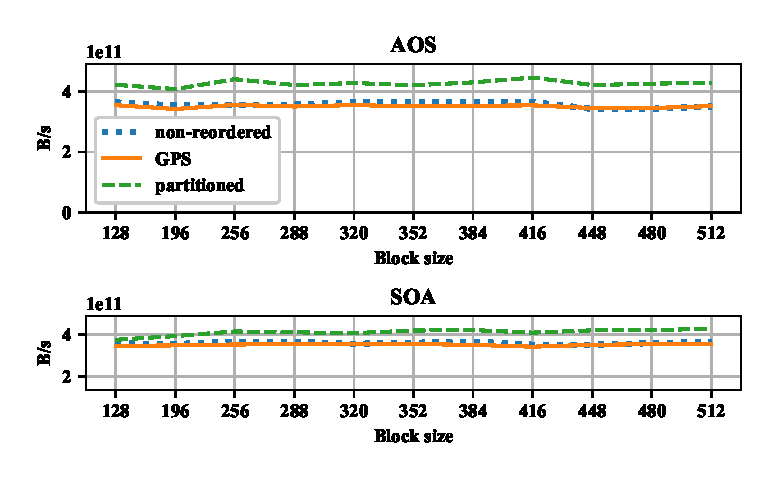
\includegraphics[width=10cm]{fig/airfoil_bw-vs-bs_hier_large_volta.eps}
\caption{Airfoil's \texttt{res\_calc} bandwidth on a dataset with $2880000$ 
cells with hierarchical colouring, on Volta architecture.} 
\label{fig:airfoil_bw-vs-bs_hier_large_volta}
\end{figure}

Similar results were obtained on the newer Volta GPUs (V100) as illustrated in 
Figure~\ref{fig:airfoil_bw-vs-bs_hier_large_volta}). The absolute value of the
bandwidths are (understandably) higher. On the V100, AOS achieved $28\%$ 
speedup in the kernel compared to the original code with $446$ GB/s bandwidth 
($60\%$ of the peak bandwidth), but the it still lacks behind SOA regarding the
whole application. The best SOA version achieved $21\%$ speedup. Since 
\texttt{res\_calc} takes around $54\%$ of the total run time this speedup lead 
to $11\%$ performance increase on the whole application.


\subsubsection{Volna}
\noindent The next application we explore here, Volna, is in fact a 
production/research code for shallow water simulation capable of handling the 
complete life-cycle of a tsunami (generation, propagation and run-up along the 
coast)~\cite{dutykh2011volna}. The simulation algorithm works on unstructured
triangular meshes and uses the finite volume method. Volna is written in C/C++
and is converted to use the OP2 library~\cite{op2-volna2018}. Volna spends 
most time in three kernels: \texttt{computeFluxes}, \texttt{SpaceDiscretization} 
and \texttt{NumericalFluxes}. Out of these, we focus on the 
\texttt{SpaceDiscretization} kernel that iterates on edges accessing data 
indirectly on cells, $60\%$ of total execution time is spent in this kernel. In 
each iteration, \texttt{SpaceDiscretization} reads 1 and increments 4 float 
values from each of the 2 indirectly accessed cells, and reads 7 float and 1 
integer values directly. A notable difference in Volna is that the execution 
with single precision is adequate for solution accuracy. As such we benchmark it 
with single precision floating-point mathematics, on a mesh containing 2.4 
million triangular cells, simulating a tsunami run-up to the US pacific coast. 

Figure~\ref{fig:volna_bw-vs-bs_hier} and Table~\ref{tab:volna_counters_hier} 
details the performance metrics observed for the \texttt{SpaceDiscretization} 
kernel in Volna. We concentrate solely on the hierarchical coloring variants 
given their superior performance to global coloring. The reordering by 
partitioning again improves performance. It increases reuse from $1.5$ to 
$2.8$ and decreases the number of global transactions by $18\%$ for reads and 
$37\%$ for writes. The larger reduction in writes can be explained by the fact 
that the calculation only reads data defined on the iteration set directly.

Again, recall that the AoS version uses adjacent threads to load adjacent 
components of data points. Additionally, given the use of single precision 
values for Volna, one thread loads $4$ single precision values into shared 
memory using the built-in vector type \lstinline!float4!. Consequently, more 
data is transferred at the same time, providing a $2\%$ and $4\%$ reduction
in global memory transfers for reads and writes, respectively. This leads 
to performance improvements of $292\,\text{GB/s}$ versus $268\,\text{GB/s}$.

Low register counts ($28$--$32$) and single-precision data types also 
resulted in achieving a higher occupancy on the GPU compared to Airfoil. This, 
we believe explains why performance appears to be independent of the block size 
as shown in the Figure \ref{fig:volna_bw-vs-bs_hier}. 

We also see that using partitioning does not increase the number of thread 
colors significantly, as we observed on Airfoil. The increase of colors are 
from $3$ to $4$. As such the overall synchronization overhead is also smaller. 
The percentage of stalls caused by synchronization increases from $12\%$ to just 
$15\%$. Of course, with high occupancy, the latency caused by synchronization 
can be better hidden by running warps from other blocks. 

%shared memory usage:
% 7.7KB, 4.3 for metis

\begin{figure}[Htbp]
  \centering
  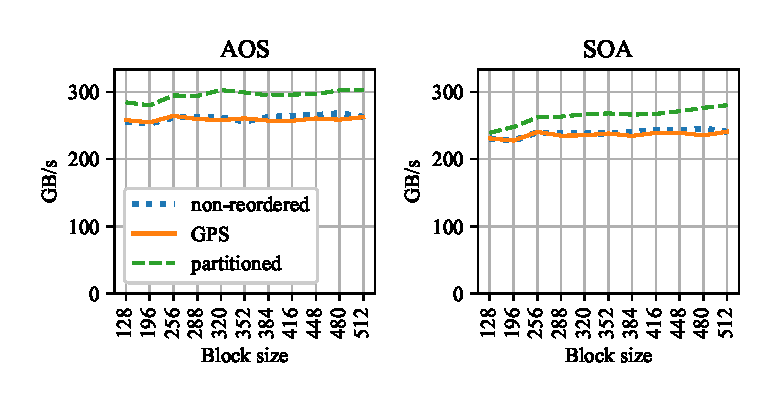
\includegraphics[width=10cm]{fig/volna_bw-vs-bs_hier.eps}
  \caption{Volna's \texttt{SpaceDiscretization} kernel bandwidth on a mesh with
  $3589735$ edges using hierarchical coloring.}
  \label{fig:volna_bw-vs-bs_hier}
\end{figure}

As can be seen in Figure \ref{fig:volna_speedup}, the locality exploiting 
optimizations makes the kernel $20\%$ faster than the original OP2 version.
Again the best performance for \texttt{SpaceDiscretization} reached with AOS 
layout which is not optimal for the whole application and the best total performance
can be reached with SOA layout. \texttt{ComputeFluxes} also benefits significantly from these optimizations since this kernel also iterates on the edges and read data from cells. We experienced $5\%$ speed increase in \texttt{ComputeFluxes}.
The increased speed of the two kernel results in a $13\%$ increase to the whole
application. The useful bandwidth also increases and reached $30\%$ of the peak
stream bandwidth of the P100 GPU.

On the V100, the performance of the kernel was $462$ GB/s ($62\%$ of the peak bandwidth) with $18\%$ (AOS) speedup. Regarding the whole application SOA 
achieved $11\%$ speedup on \texttt{SpaceDiscretization} while improving
\texttt{ComputeFluxes} with $10\%$ as well leading to a $8\%$ speedup on the
whole application compared to the original.

%XXX: make this table look more like the airfoil one


\begin{table}[Htbp]
\centering
\resizebox{\columnwidth}{!}{
\small
\begin{tabular}{|r|cc|c|c||c|}\hline
Reordering  & \multicolumn{2}{c|}{none} & \multicolumn{2}{c||}{partition} & 
original\\\hline
Data layout &    AOS      &   SOA     &     AOS      &    SOA      &    
SOA\\\hline
Bandwidth (GB/s) &   $ 133$ &   $ 120$ &   $ 146$ &   $ 134$ & $119$\\
Runtime (ms) & $0.87$ & $0.95$ & $0.77$ & $0.85$ & $0.93$\\
Achieved Occupancy &   $0.82$ &   $0.81$ &   $0.80$ &   $0.80$  &   $0.68$\\
Global Memory Read Transactions &   $ 9114\text{k}$ &   $ 9166\text{k}$ &   $ 
7493\text{k}$ &   $ 7617\text{k}$ &  $9504\text{k}$ \\
Global Memory Write Transactions &   $ 2438\text{k}$ &   $ 2512\text{k}$ &   $ 
1542\text{k}$ &   $ 1640\text{k}$ &   $ 2809\text{k}$ \\
Number of Block Colours &   $       5$ &   $       5$ &  $       9$ &   $       
9$ &   $       6$ \\
Number of Thread Colours &   $       3$ &   $       3$ &  $       4$ &   $       
4$ &   $       3$ \\
Reuse factor &   $     1.5$ &   $     1.5$ &  $     2.8$ &   $     2.8$ &   $    
 1.48$ \\
Issue Stall Reasons (Synchronization) &     $11\%$ &     $12\%$ &  $15\%$ &     
$15\%$ &     $14\%$ \\
Issue Stall Reasons (Data Request) &     $51\%$ &     $50\%$ &  $46\%$ &     
$46\%$ &     $47\%$ \\
Average cache lines/block &   $     300$ &   $     307$ &  $     165$ &   $     
184$ &   -  \\
Warp Execution Efficiency &   $  98\%$ &   $  98\%$ &   $  97\%$ &   $  97\%$ &  
 $  65\%$  \\\hline
Block size &  \multicolumn{4}{c||}{$307$} & $128$\\\hline
\end{tabular}
}
\caption{Low-level performance metrics of Volna's \texttt{SpaceDiscretization} 
kernel - hierarchical coloring. The last column details the measured performance 
of the original code.}
\label{tab:volna_counters_hier}
\end{table}


\begin{figure}[Htbp]
\centering
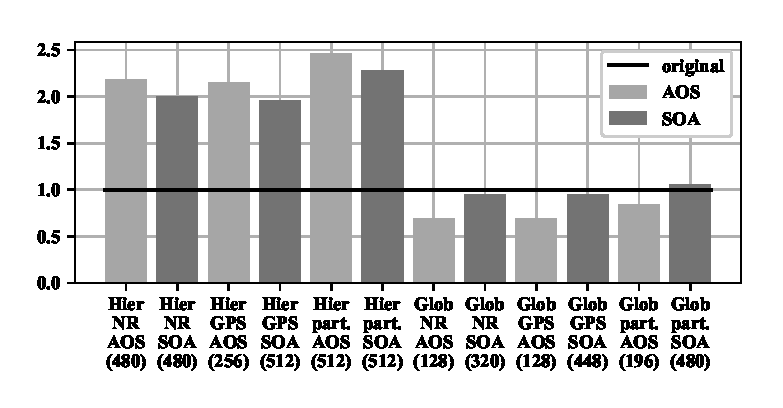
\includegraphics[width=10cm]{fig/volna_speedup.eps}
\caption{Volna's \texttt{SpaceDiscretization} kernel speedup compared to the 
original code, done on a mesh with $3589735$ edges. The block sizes are shown 
in parentheses, the reordering algorithms are: the original reordering (NR), 
GPS reordering and partitioning (part.)}
\label{fig:volna_speedup}
\end{figure}



\subsubsection{BookLeaf}
\noindent The third application we explore is BookLeaf. It is a 2D unstructured
mesh Lagrangian hydrodynamics application from the UK Mini-App Consortium
\cite{uk-mac}. It uses a low order finite element method with an arbitrary
Lagrangian-Eulerian method.  BookLeaf is written entirely in Fortran 90 and has
been ported to use the OP2 API and library. BookLeaf has a large number of
kernels with different access patterns such as indirect increments similar to
increments inside \texttt{res\_calc} in Airfoil. For benchmarking we used the
SOD test case with a mesh of 4 million cells. The top time consuming kernel with
indirect increments is \texttt{getacc\_scatter}, which iterates on cells while
incrementing data indirectly on vertices, $6\%$ of total execution time is spent
in this kernel. This kernel reads 17 double values directly, and increments 4
double values on each of the 4 indirectly accessed nodes in each iteration.

Runtime performance of BookLeaf and specifically the low-level performance of 
the \texttt{getacc\_scatter} kernel are detailed in Figures
\ref{fig:bookleaf_bw-vs-bs_hier} and \ref{fig:bookleaf_speedup}. Again we see  
benefits from partitioning. The register count and occupancy are also similar to 
those with Airfoil ($64$ registers, achieving occupancy around $40\%$), this 
now leads to the variations in performance for different block sizes. With 
partitioning, the number of thread colors increases from $2$ to $5$, this
leads to increased stalls from synchronizations: from $9\%$ to $20\%$, while
the reuse factor increases (from $2$ to $3.5$). This is comparable to 
that of Airfoil, and explains the smaller increase in performance (only $15\%$, 
compared to the $19\%$ increase in Airfoil). The higher data reuse leads to 
$14\%$ and $41\%$ decrease of the number of global transactions, for reads and 
writes, respectively. Such a large difference between reads and writes is also 
due to \texttt{getacc\_scatter} having no indirect reads, similar to 
like \texttt{SpaceDiscretization} in Volna. 

The best performance we achieved with \texttt{getacc\_scatter} ($1.15\times$ 
speedup) results in about $1\%$ performance increase for the the whole 
application. The useful bandwidth also increased and reached $83\%$ of the peak 
stream bandwidth of the P100 GPU.
On the V100, the performance of the kernel was $631$ GB/s ($85\%$ of the peak
bandwidth) which results in $0.5\%$ runtime speedup on the whole application
compared to the original.

\begin{figure}[Htbp]
\centering
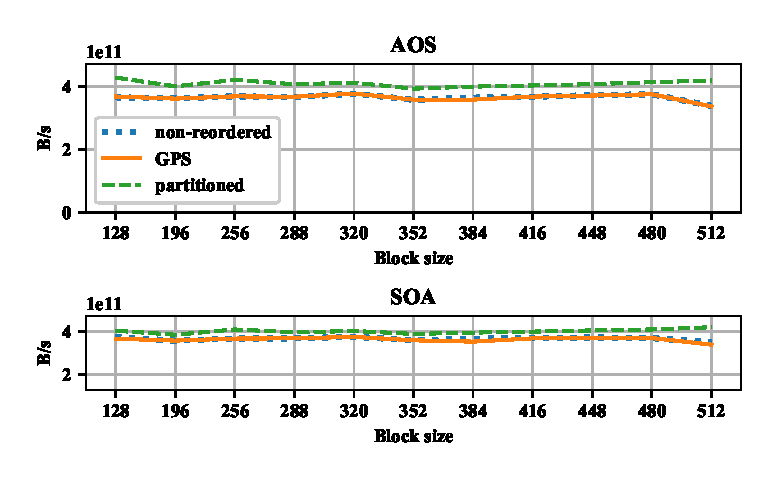
\includegraphics[width=10cm]{fig/bookleaf_bw-vs-bs_hier.eps}
\caption{Bookleaf's \texttt{getacc\_scatter} kernel bandwidth on a mesh with 
$4000000$ edges using hierarchical colouring.}
  \label{fig:bookleaf_bw-vs-bs_hier}
\end{figure}

\begin{figure}[Htbp]
\centering
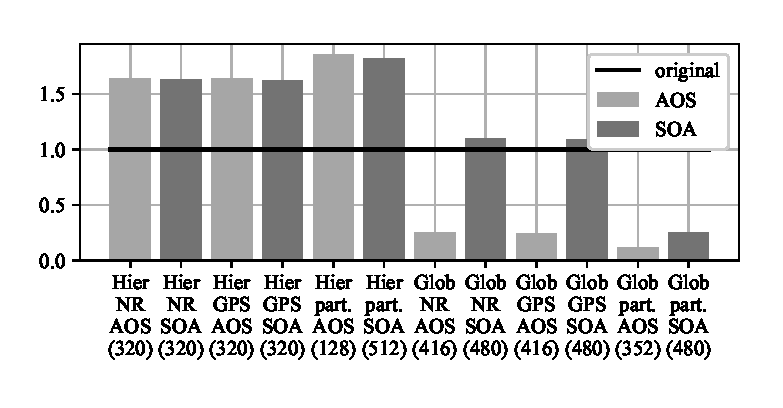
\includegraphics[width=10cm]{fig/bookleaf_speedup.eps}
\caption{Bookleaf's \texttt{getacc\_scatter} kernel speedup compared to the 
original code, done on a mesh with $4000000$ edges. The block sizes are shown 
in parentheses, the reordering algorithms are: the original reordering (NR), 
GPS reordering and partitioning (part.)}
  \label{fig:bookleaf_speedup}
\end{figure}


\subsubsection{LULESH}\label{sec:lulesh-summary}

\hyphenation{CalcFBHourglassForceForElems IntegrateStressForElems}

\noindent LULESH (Livermore Unstructured Lagrangian Explicit Shock 
Hydrodynamics~\cite{LULESH2:changes}) application represents a typical 
hydrocode representing the Shock Hydrodynamics Challenge Problem that was 
originally defined and implemented by Lawrence Livermore National Lab as one of 
five challenge problems in the DARPA UHPC program. It  has since become a widely 
studied proxy application in DOE co-design efforts for exascale. 

LULESH is a highly simplified application, hard-coded to only solve a simple
Sedov blast problem that has an analytic solution~\cite{LULESH:spec} – but
represents the numerical algorithms, data motion, and programming style typical
in scientific C/C++ based applications at the Lawrence Livermore National
Laboratory. LULESH approximates the hydrodynamics equations discretely by
partitioning the spatial problem domain into a collection of volumetric elements
defined by a mesh. The mesh itself is structured (and generated in the code), 
but the algorithm doesn't take this into account and accesses the data through 
an eight-dimensional mapping for the hex8 (brick) elements.

We explore the \texttt{IntegrateStressForElems} kernel that calculates the
forces in the nodes. Iterating over cells, it reads 3 double values from each 
of the 8 indirectly accessed nodes, increments 3 double values for each node, 
reads 3 double values directly and writes 1 double value directly. In our 
measurements, we used a mesh with \num{4913000} cells and \num{5000211}
nodes. The original CUDA version of the code contracted this kernel with
\texttt{CalcFBHourglassForceForElems}; the only modifications we applied to 
this code for our tests was to remove these parts from the kernel.

The \texttt{IntegrateStressForElems} kernel uses a mapping with 8 neighbors for 
the brick elements (compared to the 2--4 as in the case of the previous 
application kernels). As a result, the number of block colors is quite high: $8$, $16$ 
and $24$ in the global coloring versions (for the different reorderings), and 
$4$, $5$ and $15$ in the hierarchical coloring versions. The number of thread 
colors was also quite high: $4$ in the non-reordered ($4.5$ in the GPS) and 
$11.6$ in the partitioned version. The non-reordered and GPS versions yield 
blocks that have ``pencil shape'', thus requiring fewer thread colors, whereas 
the partitioned version yields more cubical shaped blocks, leading to the higher 
number of thread colors. This is a much larger increase compared to the previous 
applications (Table~\ref{tab:lulesh_counters_hier}). At the same time of course, 
data reuse is higher compared to 2D applications - between $2.6$ and $4.8$.

The other aspect in which LULESH is differs is that it uses a high amount of
registers ($96$), which significantly decreases occupancy: with block size 320, 
the AoS version achieved $15\%$ and the SoA version achieved around $30\%$. 
Because of these two reasons, the synchronization overhead ($39\%$ stalls were 
from synchronization on the partitioned mesh) couldn't be hidden: there were no 
warps from other blocks to be scheduled in place of the stalled ones because
there was only one block running on each multiprocessor. The difference in 
achieved occupancy also means that the SoA version with two blocks 
per multiprocessor gives better performance.

The original implementation used either atomics or helper arrays as a means of
avoiding data races. As shown in Figure \ref{fig:lulesh_speedup}, the
hierarchical coloring algorithm performs significantly better (giving a $49\%$
speedup) than the original two-step implementation (and also uses much less
memory), but it is worse than the original atomics implementation by $17\%$.

% Although the original requires less synchronization, the resulting warp
% divergence also cannot be hidden if the occupancy is this low.
 
\begin{figure}[Htbp]
\centering
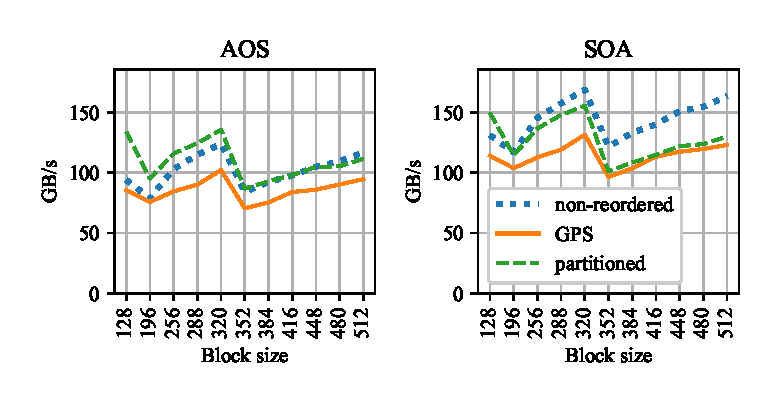
\includegraphics[width=10cm]{fig/lulesh_bw-vs-bs_hier.eps}
\caption{LULESH's \texttt{IntegrateStressForElems} kernel bandwidth on a mesh 
with $4913000$ cells using hierarchical colouring.}
  \label{fig:lulesh_bw-vs-bs_hier}
\end{figure}

In the original application version $37\%$ out of the total time is spent in
the \texttt{IntagrateStressForElems} kernel, therefore the achieved $49\%$
speedup on the kernel over the two-step implementation gives about $11\%$ (for
our best result) or $8\%$ (for our partitioned version) speedup on the whole
application. This was measured by reading back the reordered mesh in the
original code for all kernels. The useful bandwidth in case of the best version
of \texttt{IntegrateStressForElems} reached $35\%$ of the peak stream bandwidth
on the P100 GPU.

On the V100, we achieved $51\%$ speedup for this kernel compared to the original
two-step implementation with $270$ GB/s bandwidth ($36\%$ of the peak
bandwidth). In the original version $38\%$ of the total time is spent in
\texttt{IntegrateStressForElems}, therefore this achieved kernel speedup results
in about $16\%$ speedup on the whole application. Again, the atomics version
performed best with a bandwidth of $561$ GB/s ($76\%$ of peak bandwidth), two
times faster than our version.

\begin{figure}[Htbp]
\centering
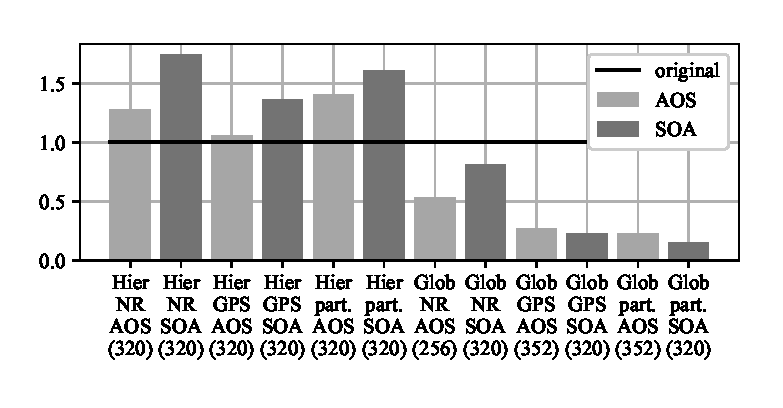
\includegraphics[width=10cm]{fig/lulesh_speedup.eps}
\caption{LULESH's \texttt{IntegrateStressForElems} kernel speedup compared to
  the original (gathering) code, done on a mesh with $4913000$ cells. The block
  sizes are shown in parentheses, the reordering algorithms are: the original
  reordering (NR), GPS reordering and partitioning (part.) The last bar shows
  the relative performance of the original code with the helper array
  approach.}
\label{fig:lulesh_speedup}
\end{figure}

\begin{table}[Htbp]
  \centering
  \resizebox{\columnwidth}{!}{
  % \begin{tabular}{|R{2.5cm}|cc|c|c|}
    \small
  \begin{tabular}{|r|cc|c|c||c|}
    \hline
      Reordering  & \multicolumn{2}{c|}{none} & \multicolumn{2}{c||}{partition} 
& original\\
      \hline
      Data layout &    AOS      &   SOA     &     AOS      &    SOA & SOA\\
      \hline
                               Bandwidth (GB/s) &   $ 80$ &   $ 172$ &   $ 83$ 
&   $ 157$ & $97$\\
                               Runtime (ms)     &   $8.48$ & $3.90$ & $8.10$ & 
$4.31$ & $6.98$ \\
                             Achieved Occupancy &   $0.15$ &   $0.29$ &   $0.15$ 
&   $0.30$ & $0.24$\\
        Global Memory Read Transactions (total) &   \num{33546}k & \num{35395}k 
&   \num{22883}k &   \num{25006}k  & \num{16072}k\\
       Global Memory Write Transactions (total) &   \num{12674}k & \num{12706}k 
&   \num{ 8052}k &   \num{ 8703}k  & \num{32689}k\\
                        Number of Block Colours &   $       4$ &   $       4$ & 
$      15$ &   $      15$ & - \\
                       Number of Thread Colours &   $       4$ &   $       4$ & 
$    9.8$ &   $    9.8$  & -\\
                                   Reuse Factor &   $     2.6$ &   $     2.6$ & 
$     4.8$ &   $     4.8$ & -\\
          Issue Stall Reasons (Synchronization) &   $  13\%$ &   $  19\%$ &   $ 
36\%$ &   $  39\%$  & $0\%$\\
             Issue Stall Reasons (Data Request) &   $  63\%$ &   $  56\%$ &   $ 
38\%$ &   $  34\%$  & $26\%$\\
                      Average Cache Lines/Block &   $     744$ &   $     747$ & 
$     427$ &   $     474$  & -\\
                      Warp Execution Efficiency &   $  98\%$ &   $  98\%$ &   $ 
94\%$ &   $  93\%$ & $100\%$\\
      \hline
      Block size & \multicolumn{4}{c||}{$320$} & $64$\\

    \hline
  \end{tabular}
  }
\caption{Low-level performance metrics of LULESH's 
\texttt{IntegrateStressForElems} kernel - hierarchical coloring. The last column 
details the measured performance of the original kernel.}  
\label{tab:lulesh_counters_hier}
\end{table}

\subsubsection{miniAero}\label{sec:mini-aero-summary}

The final application we explore is miniAero \cite{miniaero}, which is a 
mini-application from the Mantevo suite \cite{heroux2009improving}. MiniAero is 
an explicit (4th order Runge-Kutta) unstructured finite volume code that solves 
the compressible Navier-Stokes equations. Both inviscid and viscous terms are 
included. The viscous terms can be optionally included or excluded. For 
miniAero, meshes are created within the code and are simple 3D hex8 meshes. 
These meshes are generated on the CPU and then moved to the GPU. While 
the meshes generated in code are structured, the code itself uses unstructured 
mesh data structures and access patterns. This mini-application uses the Kokkos 
library~\cite{CarterEdwards20143202}.

For miniAero we study the \texttt{compute\_face\_flux} kernel that computes the
flux contributions of the faces and increments it with the appropriate cell flux
values. The kernel iterates over the faces of the mesh, and accesses the cells
indirectly. In each iteration, it reads 28 and increments 5 double values from
each of the 2 indirectly accessed cells, and reads 12 double values directly. 
The original code, depending on a compile time parameter, either uses 
the auxiliary \texttt{apply\_cell\_flux} kernel that does the actual 
incrementing by gathering the intermediate results from a large temporary array, 
or uses atomics to do it within the kernel. Both the atomics and the work of 
the auxiliary kernel was substituted in our code by coloring.


% results


The \texttt{compute\_face\_flux} kernel is the most computationally intensive
among the ones we tested: it uses $165$ registers in hierarchical coloring
($166$ in SoA layout). Also, it achieves, with a block size of $384$ and 
reordered by GPS, $15\%$ of peak double precision efficiency, compared to the 
$6$--$7\%$ in Airfoil (Table \ref{tab:mini_aero_counters_hier}). It also uses 
$8$ square root operations and several divides that can't efficiently fill the 
pipelines at such low occupancy. 

The amount of data indirectly accessed by the kernel is also significant: each 
thread accesses $2$ data points indirectly, each holding $32$ double precision 
values. If all of these values are loaded into shared memory, the size exceeds 
the hardware limits with block sizes larger than $288$; it didn't run with the 
original mesh numbering with any block size, and only with smaller block sizes 
on the reordered meshes (Figure \ref{fig:mini_aero_bw_crash}). The other 
measurements were carried out by only loading the incremented data into shared 
memory.

\begin{figure}[Htbp]
\centering
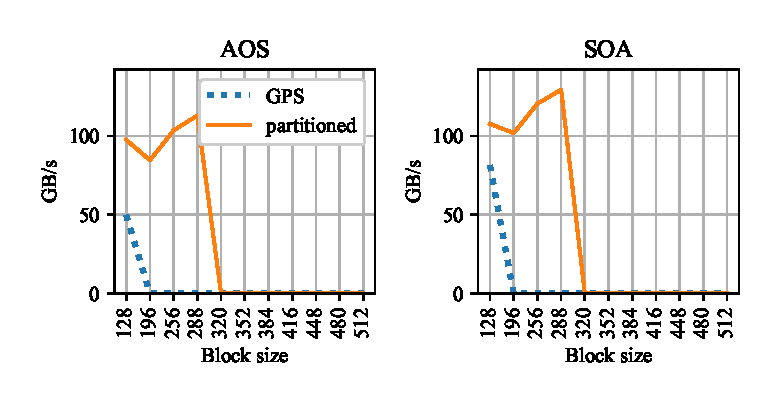
\includegraphics[width=10cm]{fig/mini_aero_bw_crash.eps}
\caption{miniAero's \texttt{compute\_face\_flux} kernel bandwidth on a mesh 
with $6242304$ faces. The kernel didn't run in the cases where the data reuse 
was not high enough because the large amount of shared memory needed; these 
are shown here with $0$ bandwidth.}
  \label{fig:mini_aero_bw_crash}
\end{figure}

The mesh also has a complex structure. $18$ and $15$ block colors for the GPS
reordered and partitioned versions, respectively. The original ordering was
far from optimal, we couldn't run the non-reordered version, because the 
number of block colors exceeded the implementation limit of the library, which 
is $256$. As with LULESH, only one block was running at a time on each 
multiprocessor. Although the synchronization overhead was lower ($3$ and $6$ 
thread colors in the GPS reordered and partitioned versions, respectively), the 
costly operations prevented high performance gains in the case of the 
partitioned version (Figure \ref{fig:mini_aero_bw_small-cache}).

\begin{figure}[Htbp]
\centering
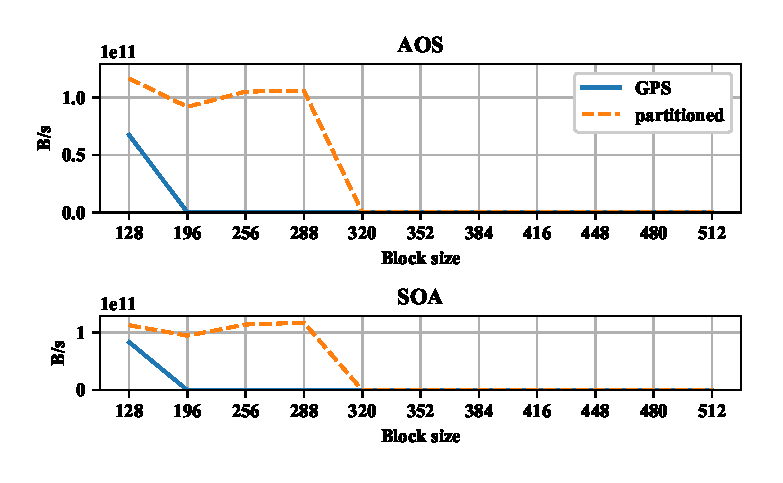
\includegraphics[width=10cm]{fig/mini_aero_bw_small-cache.eps}
\caption{miniAero's \texttt{compute\_face\_flux} kernel bandwidth on a mesh 
with $6242304$ faces. The shared memory was only used to cache the increments,
reducing the need for large shared memory size. The kernel didn't fit into the
shared memory with block sizes larger than $384$ or if not reordered because
the large amount of shared memory needed; these are shown here with $0$
bandwidth.} \label{fig:mini_aero_bw_small-cache}
\end{figure}

The original Kokkos implementation either used atomic adds or the two-step
gathering approach depending on compilation parameters. Our implementation
outperformed both with a 75\% speedup (Figure
\ref{fig:mini_aero_speedup_small-cache}). In the original version $22\%$ of the
total time is spent in \texttt{compute\_face\_flux}, therefore the achieved
$75\%$ kernel speedup provides about $10\%$ speedup for the whole application.
When measuring on the reordered mesh for all kernels (substituting the above
speedup for \texttt{compute\_face\_flux}), the performance actually decreases to
$84\%$ of the original.  The useful bandwidth in case of the best version of
\texttt{compute\_face\_flux} ($168$ GB/s) reached $34\%$ of the peak stream
bandwidth of the P100 GPU.

\begin{figure}[Htbp]
\centering
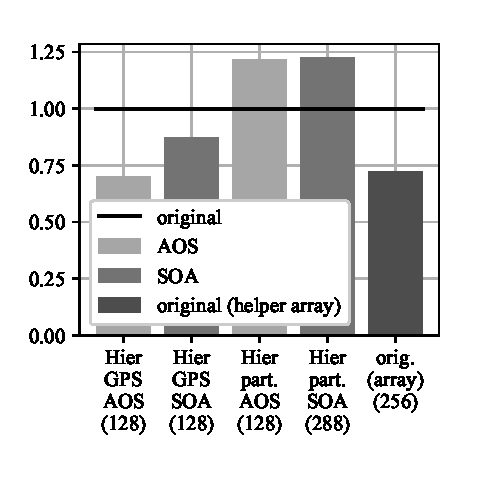
\includegraphics[width=10cm]{fig/mini_aero_speedup_nocache.eps}
\caption{miniAero's \texttt{compute\_face\_flux} kernel speedup compared to 
the original code that was using atomic adds, on a mesh with $6242304$ faces. 
The shared memory was only used to cache the increments, reducing the need 
for large shared memory size. The last bar shows the relative performance of 
the original code with the helper array approach.}
\label{fig:mini_aero_speedup_small-cache}
\end{figure}

\begin{table}[Htbp]
  \centering
  \resizebox{\columnwidth}{!}{
    \small
  % \begin{tabular}{|R{2.5cm}|cc|c|c|}
  \begin{tabular}{|r|cc|c|c||c|}
    \hline
      Reordering  & \multicolumn{2}{c|}{GPS} & \multicolumn{2}{c||}{partition} & 
original\\
      \hline
      Data layout &    AOS      &   SOA     &     AOS      &    SOA & SOA\\
      \hline
                               Bandwidth (GB/s)&    $  67$ &   $ 84$ &   $ 117$ 
&   $ 113$ & $96$\\
                               Runtime (ms)    &    $19.09$ & $15.38$ & $11.04$
                               & $11.38$ & $13.39$\\
                             Achieved Occupancy&    $0.06$ & $0.06$ & $0.12$ & 
$0.12$  & $0.23$\\
                Global Memory Read Transactions&    $73561\text{k}$ & 
$82028\text{k}$ & $53403\text{k}$ & $77091\text{k}$  & $87368\text{k}$\\
               Global Memory Write Transactions&    $9153\text{k}$ & 
$10390\text{k}$ & $6694\text{k}$ & $9008\text{k}$ & $5934\text{k}$ \\
                        Number of Block Colours&    $      18$ &   $      18$ & 
$      15$ &   $      15$  & -\\
                       Number of Thread Colours&    $       3$ &   $       3$ & 
$       6$ &   $       6$  & -\\
                                   Reuse Factor&    $     2.2$ &   $     2.2$ & 
$     3.9$ &   $     3.9$  & -\\
          Issue Stall Reasons (Synchronization)&    $4\%$ & $9\%$ & $15\%$ & 
$21\%$    & $0\%$ \\
             Issue Stall Reasons (Data Request)&    $61\%$ & $35\%$ & $47\%$ & 
$35\%$  & $49\%$\\
     Issue Stall Reasons (Execution Dependency)&    $23\%$ & $33\%$ & $23\%$ & 
$23\%$  & $13\%$\\
                      Average Cache Lines/Block&    $     452$ &   $     471$ & 
$     269$ &   $     344$  & -\\
                      Warp Execution Efficiency&    $91\%$ & $84\%$ & $88\%$ & 
$85\%$  & $91\%$\\
                   FLOP Efficiency(Peak Double)&    $5\%$ & $8\%$ & $10\%$ & 
$12\%$  & $8\%$\\
      \hline
      Block size & \multicolumn{4}{c||}{128} & 256\\
    \hline
  \end{tabular}
  }
\caption{ Low-level performance metrics of the miniAero's 
\texttt{compute\_face\_flux} kernel - hierarchical coloring. The last column 
details the measured performance of the original code.}
  \label{tab:mini_aero_counters_hier}
\end{table}

On Volta, we achieved $158\%$ (compared to the atomic version) and $92\%$
(compared to the two-step version) speedups in the kernel $268$ GB/s bandwidth
($36\%$ of the peak bandwidth). In the original version $19\%$ of the total time
is spent in \texttt{compute\_face\_flux}, therefore the kernel speedup
provides about $13\%$ and $10\%$ speedups for the whole application (compared
to the atomic and the two-step versions, respectively).

When measured with all kernels reordered, the performance again decreases, by
$27\%$ compared to the original two-step implementation.


\subsubsection{Analysis of structured meshes}
\label{analysis-of-structured-meshes}

\noindent Recalling that the meshes of miniAero and LULESH are actually 
structured meshes, generated by the code itself allows us to use their 
structured nature to create partitions with better shapes as opposed to 
partitions produced by METIS. This in turn allows us to understand the trade-off 
between high data reuse and number of thread colors.  We create 1D (straight 
line), 2D (rectangles) and 3D (bricks) shape partitions such that these will 
have an increasing amount of reuse, and with that, number  of colors. 

While both kernels operate on 3D Cartesian (hex8) meshes, the LULESH kernel 
\texttt{IntegrateStressForElems} uses a mapping from cells to their connected 
vertices, and the \texttt{compute\_face\_flux} kernel in miniAero maps from 
(internal) faces to cells. We created a number of different partition shapes - 
1D lines, 2D rectangles and 3D bricks. Figures~\ref{fig:lulesh_block} and 
\ref{fig:mini_aero_block} show the bandwidths, reuse factors and the number of 
thread colors across different block-shapes, along with the result of 
partitioning the same mesh using METIS. The size of the blocks is $128$. The 
results are from meshes with specifically tailored shapes so that the 
handcrafted blocks can cover them without any gaps. 

In \texttt{IntegrateStressForElems}, the achieved bandwidth of the 
original ordering is $134\,\text{GB/s}$ - it uses a row major order. This is 
similar to what we use for a line block shape that is $128$ cells long and only $1$ 
cell thin in the other dimensions. The partitioned mesh (as detailed in Section 
\ref{sec:lulesh-summary}) achieved $132\,\text{GB/s}$, and we achieved 
$167\,\text{GB/s}$ bandwidth using our handcrafted blocks, for the same block 
size ($128$). Note that using regular shapes is better for the thread coloring 
algorithm as well. With METIS partitioning, the number of colors needed 
is higher than in the other cases.

For \texttt{compute\_face\_flux}, we achieved $167\,\text{GB/s}$ bandwidth,
compared to $101\,\text{GB/s}$ achieved with METIS partitioning. Of course, 
using these handcrafted blocks can only be done on meshes that are actually 
structured, therefore this is not representative of realistic cases. However, 
these results illustrate clearly that when the number of thread colors are the 
same, increased reuse leads to better performance. Also, there is an optimal 
trade off between reuse and the number of thread colors for each application, 
and performance will suffer above/below that. As an alternative to METIS, we 
explored using SCOTCH~\cite{Pellegrini1996} to create the required partitions. 
However SCOTCH also did not produce a better partitioning for these 
applications. The challenge lies in finding a partitioning algorithm that can 
either find the middle ground, or can be tuned  along the amount of reuse it 
aims to achieve. Such partitioning algorithms are not currently available, but 
the evidence here clearly demonstrate their usefulness. 


\begin{figure}[Htbp]
\centering
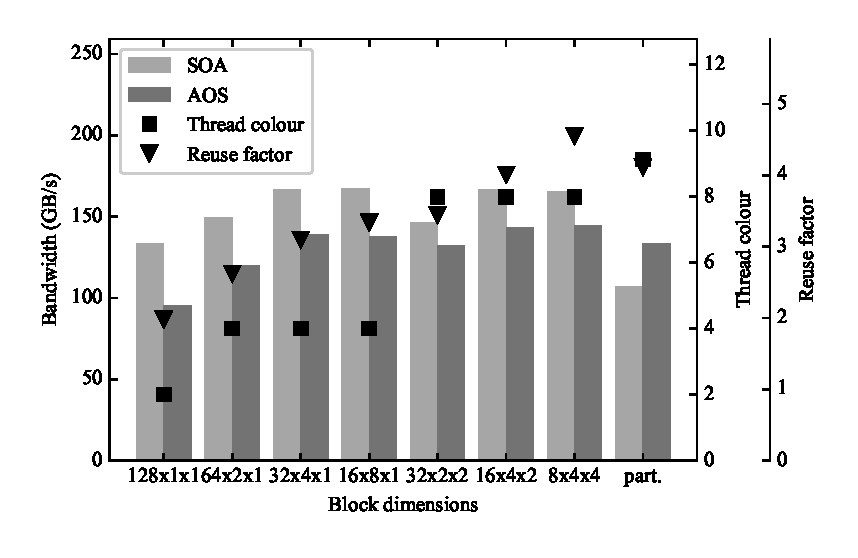
\includegraphics[width=12cm]{fig/lulesh_block.eps}
\caption{LULESH's \texttt{IntegrateStressForElems} kernel with explicitly 
controlled partitioning. For comparison, the last column shows the result on 
the same mesh, partitioned by METIS.} \label{fig:lulesh_block}
\end{figure}

\begin{figure}[Htbp]
\centering
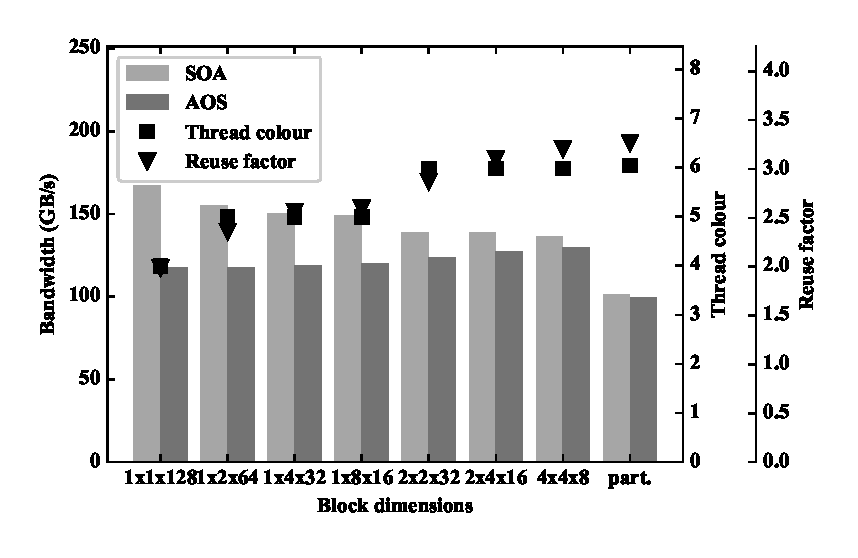
\includegraphics[width=12cm]{fig/mini_aero_block.eps}
\caption{miniAero's \texttt{compute\_face\_flux} kernel with explicitly 
controlled partitioning. For comparison, the last column shows the result on 
the same mesh, partitioned by METIS.} \label{fig:mini_aero_block}
\end{figure}
